\chapter*{Задание №4}
Задание: предок и потомки обмениваются сообщениями через неименованный программный канал. Причем оба потомка пишут свои сообщения в один программный канал, а предок их считывает из канала. Потомки должны посылать предку разные сообщения по содержанию и размеру. Предок считывает сообщения от потомков и выводит их на экран. Предок ждет завершения своих потомков и анализирует код их завершения. Вывод соответствующих сообщений на экран.

\begin{lstlisting}[label = exec, caption=Обмен сообщениями предка и потомка через неименованный программный канал.]
#include <unistd.h>
#include <stdio.h>
#include <sys/wait.h>
#include <string.h>

#define FORK_ERROR -1
#define FORK_OK 0
#define BUFFER_SIZE 256

#define COUNT_CHILDS 3

int main(void)
{
	pid_t childs_pid[COUNT_CHILDS];
	pid_t child_pid;
	
	int file_descriptors[2];
	const char *messages[COUNT_CHILDS] = {"gegwege\n", "fwgrzdjnkfjrbgegb\n", "ng\n"};
	char buffer[BUFFER_SIZE] = {0};
	
	int res_exec = 0;
	
	pipe(file_descriptors);
	
	printf("Parent - pid: %d, pgrp: %d\n", getpid(), getpgrp());
	
	for (int i = 0; i < COUNT_CHILDS; i++)
	{
		child_pid = fork();
		if (child_pid == FORK_ERROR)
		{
			perror("Can't fork.\n");
			return 1;
		}
		else if (child_pid == FORK_OK)
		{
			close(file_descriptors[0]);
			write(file_descriptors[1], messages[i], strlen(messages[i]));
			printf("Message from child_%d sent to the parent.\n", i + 1);
			
			return 0;
		}
		else{
			childs_pid[i] = child_pid;
		}
		
	}
	
	for (int i = 0; i < COUNT_CHILDS; i++)
	{
		int status;
		pid_t child_pid = wait(&status);
		
		printf("Child has finished - pid: %d, ppid = %d\n", child_pid, getppid());
		
		if (WIFEXITED(status)){
			printf("Child exited with code %d\n", WEXITSTATUS(status));
		}
		else {
			printf("Child terminated abnormally.\n");
		}
	}
	
	
	close(file_descriptors[1]);
	read(file_descriptors[0], buffer, BUFFER_SIZE);
	
	printf("Received message:\n%s", buffer);
	
	printf("Parent - child_1_pid: %d, child_2_pid: %d, child_3_pid: %d\n", childs_pid[0], childs_pid[1], childs_pid[2]);
	printf("Parent process is dead\n");
	
	return 0;
}

\end{lstlisting}


Результат работы программы представлен на рисунке \ref{png:res_4}:

\begin{figure}[H]
	\centering{
		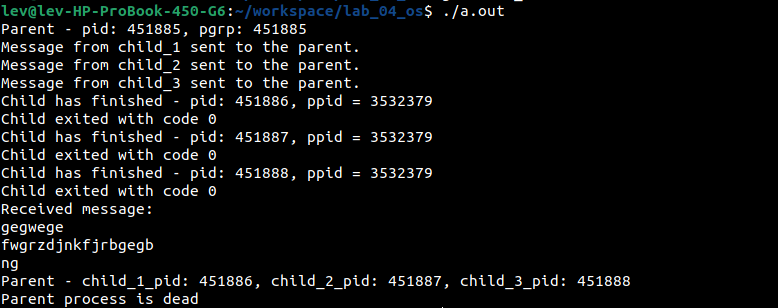
\includegraphics[scale=0.5]{../../../../../../../msys64/home/Лев/bmstu_sem_5_os/lab_04/report/images/task_4}
		\caption{Демонстрация работы программы (задание 4).}
		\label{png:res_4}}
\end{figure}